\chapter{First order transition Hamiltonian}
First order transition Hamiltonian can be written in a form
\begin{equation}
    \HH=\J_3-\frac{\tilde\lambda(t)}{2j}\left(\J_1+\tilde\chi(\J_3+j\Id)\right)^2
    \label{eq:firstOrderTransitionHamiltonianOriginal}
\end{equation}
for $\J=(\J_1,\J_2,\J_3)$ angular momentum operator, $\tilde\chi\in\R$ and $\tilde\lambda(t)$ some real time dependent parameter. The aim is to diagonalize this Hamiltonian to find the spectrum. To make driving parameters less entwined, we will instead use the Hamiltonian
\begin{equation}
    \HH=\J_3+\lambda\hat V_1 +\chi \hat V_2+\chi^2 \hat V_3,
    \label{eq:firstOrderTransitionHamiltonian}
\end{equation}
for
\begin{align}
    \hat V_1 &=-\frac{1}{2j}\J_1^2\\
    \hat V_2 &= -\frac{1}{2j}\left[\J_1(\J_3+j)+(\J_3+j)\J_1\right]\\
    \hat V_3 &= -\frac{1}{2j}(\J_3+j)^2
\end{align}



Using the eigenbasis $\{\ket{j,m}\}$ for $j$ angular momentum quantum number and $m$ its projection to the direction $\J_3$ and defining
\begin{equation}
    \J_\pm\coloneqq\frac{1}{2}(\J_1\pm i\J_2),
\end{equation}
we get matrix elements
\begin{align}
    \braket{j'm'|\J^2|jm} &= j(j+1)\delta_{j'j}\delta_{m'm}\\
    \braket{j'm'|\J_3|jm} &= m \delta_{j'j}\delta_{m'm}\\
    \braket{j'm'|\J_\pm|jm} &= \sqrt{(j\mp m)(j\pm m+1)}\delta_{j'j}\delta_{m'm\pm 1},
\end{align}
where $\delta_{a'b}$ is Kronecker delta. Using
\begin{align}
        \left(\J_1+\chi(\J_3+j)\right)^2 &= \textcolor{purple}{\J_1^2} +\chi^2 (\J_3^2+j^2\Id+2j\J_3)+\chi(\textcolor{blue}{\J_1}\J_3+\J_3\textcolor{blue}{\J_1})+2\chi j\textcolor{blue}{\J_1}\\
        \textcolor{purple}{\J_1^2}&= \frac{1}{4}(\J_++\J_-)^2= \frac{1}{4}(\J_+^2+\J_-^2+\textcolor{violet}{\J_+\J_-}+\textcolor{violet}{\J_-\J_+})\\ 
        \textcolor{violet}{\J_\pm\J_\mp}&=\J^2-\J_3^2 \mp \J_3\\
        \textcolor{blue}{\J_1}&=(\J_+ +\J_-),
\end{align}
we get pentadiagonal matrix representation of $\HH$.
% \begin{equation}
%     \HH=\begin{pmatrix}
%         h_a   &h_b   &h_c   &0     &\dots &0\\
%         h_b   &\ddots&\ddots&\ddots&\ddots&\vdots\\
%         h_c   &\ddots&\ddots&\ddots&\ddots&0\\
%         0     &\ddots&\ddots&\ddots&\ddots&h_c\\
%         \vdots&\ddots&\ddots&\ddots&\ddots&h_b\\
%         0     &\dots &0     &h_c   &h_b   &h_a\\
%     \end{pmatrix}
% \end{equation}


\section{Hamiltonian analysis}


\subsection{Case N=3}
The lowest dimension with characteristics common to higher $N$ is 3 with Hamiltonian in eigenbasis
\begin{equation}
    \HH=\left(
        \begin{array}{cccc}
         -\frac{ \lambda +6}{4} & -\frac{\chi }{2 \sqrt{3}} & -\frac{\lambda }{2 \sqrt{3}} & 0 \\
         -\frac{\chi }{2 \sqrt{3}} & \frac{ \left(-7 \lambda -4 \chi ^2-6\right)}{12} & -\chi  & -\frac{\lambda }{2 \sqrt{3}} \\
         -\frac{\lambda }{2 \sqrt{3}} & -\chi  & \frac{ \left(-7 \lambda -16 \chi ^2+6\right)}{12} & -\frac{5 \chi }{2 \sqrt{3}} \\
         0 & -\frac{\lambda }{2 \sqrt{3}} & -\frac{5 \chi }{2 \sqrt{3}} & -\frac{\lambda }{4}-3 \chi ^2+\frac{3}{2} \\
        \end{array}
        \right).
\end{equation}
Spectrum of this Hamiltonian can be written in analytically using some substitutions $A,B,C,D$, see Appendix \ref{appendix1}, as
\begin{align}
        E_0 &= \frac{1}{12} \left(G-F-\frac{\sqrt{D-E}}{2}\right)
        \label{eq:N=3_en0}\\
        E_1 &= \frac{1}{12}  \left(G-F+\frac{\sqrt{D-E}}{2}\right)
        \label{eq:N=3_en1}\\
        E_2 &= \frac{1}{12} \left(G+F-\frac{\sqrt{D+E}}{2}\right)
        \label{eq:N=3_en2}\\
        E_3 &= \frac{1}{12}  \left(G+F+\frac{\sqrt{D+E}}{2}\right).
        \label{eq:N=3_en3}
\end{align}

Sections $\lambda=1$ and $\chi=1$ are shown in figures \ref{fig:N=3_energiesl},\ref{fig:N=3_energiesc}
\begin{figure}[h]
    \centering
    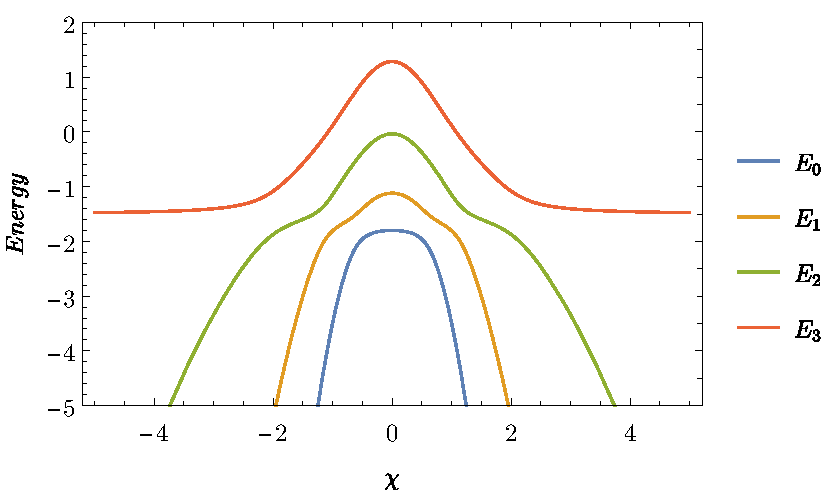
\includegraphics{../img/N=3_energiesl.pdf}
    \caption{Energy for the case $N=3$ Hamiltonian, section $\lambda=1$}
    \label{fig:N=3_energiesl}
\end{figure}
\begin{figure}[h]
    \centering
    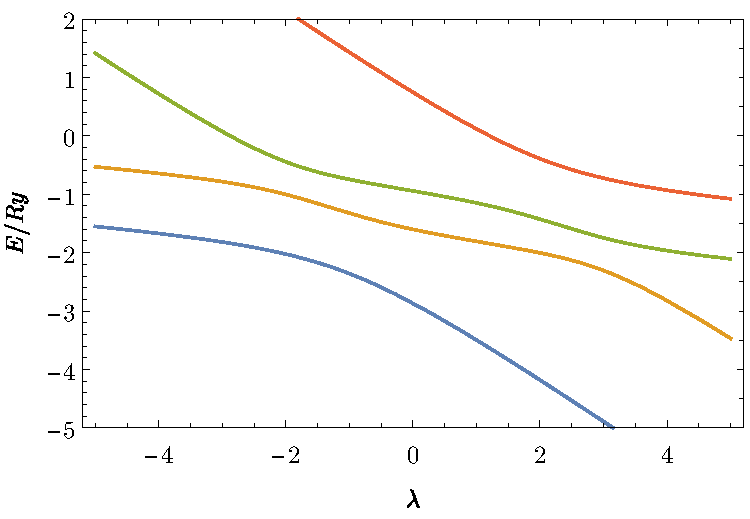
\includegraphics{../img/N=3_energiesc.pdf}
    \caption{Energy for the case $N=3$ Hamiltonian, section $\chi=1$}
    \label{fig:N=3_energiesc}
\end{figure}

From equations \ref{eq:N=3_en0}, \ref{eq:N=3_en1} can be seen that $E_0=E_1$ for $D=E$, which for real values $\lambda,\;\chi$ has two solutions
$$(\lambda_d,\pm \chi_d)=\left(-\frac{1}{2},\pm\sqrt{\frac{3}{5}}\right).$$
The solution is point-like, because we only care about real solutions. Further on, this corresponds to Theorem \ref{thm:n-2}, which states that Hamiltonian driven by two real parameters can be degenerated only on 0-dimensional manifolds.


Here the energy spectrum is degenerate and metric tensor diverges, see fig. \ref{fig:N=3_gDivenrgence}, along with Christoffel symbols elements, see fig. \ref{fig:N=3_G}. Note that metric tensor determinant is positive definite, thus the manifold is Riemannian.
\begin{figure}[h]
    \centering
    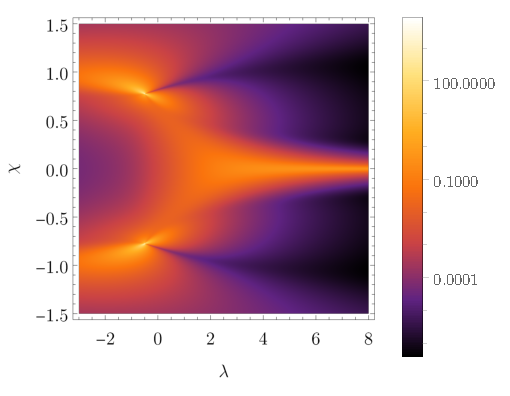
\includegraphics{../img/N=3_gDivergence.pdf}
    \caption{Arcustangens of the metric determinant in a parametric space for $N=3$.}
    \label{fig:N=3_gDivenrgence}    
\end{figure}

\begin{figure}
    \centering
    \begin{tabular}{cc}
    \subcaptionbox{$\arctan(\Gamma_{111})$}{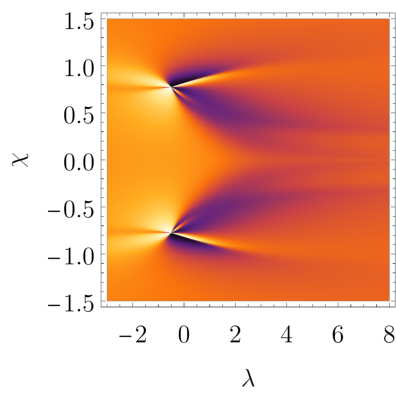
\includegraphics{../img/N=3_G111.pdf}} &
    \subcaptionbox{$\arctan(\Gamma_{211})$}{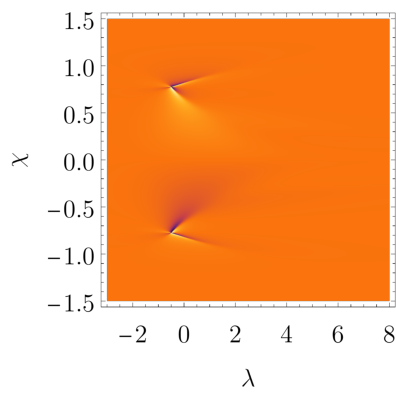
\includegraphics{../img/N=3_G211.pdf}} \\
    \subcaptionbox{$\arctan(\Gamma_{121})$}{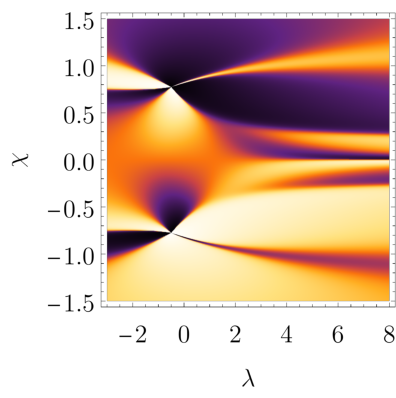
\includegraphics{../img/N=3_G121.pdf}} &
    \subcaptionbox{$\arctan(\Gamma_{221})$}{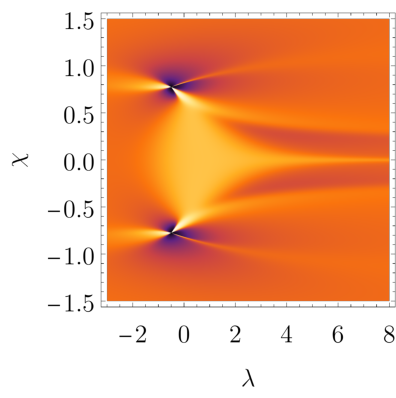
\includegraphics{../img/N=3_G221.pdf}}\\
    \subcaptionbox{$\arctan(\Gamma_{122})$}{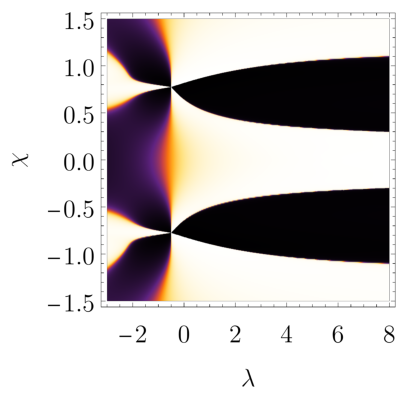
\includegraphics{../img/N=3_G122.pdf}} &
    \subcaptionbox{$\arctan(\Gamma_{222})$}{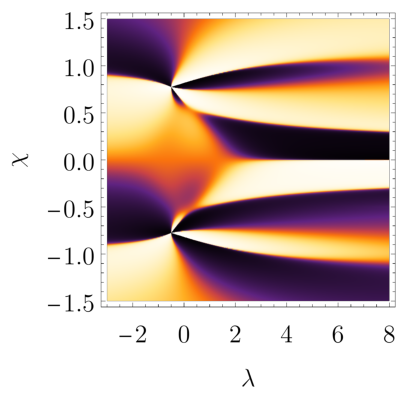
\includegraphics{../img/N=3_G222.pdf}}\\
    \end{tabular}
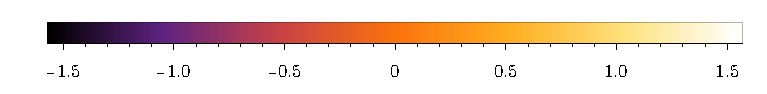
\includegraphics{../img/N=3_barA.pdf}
    \caption{Arcustangens of Christoffel symbols for the case $N=3$}
    \label{fig:N=3_G}
\end{figure}

Due to metric tensor degeneracy, the space is not geodesically complete and according to \ref{thm:hopf-Rinow_modified} there exist some "event horizon" around singularities $(\lambda_d,\pm \chi_d)$. This can be seen more clearly from geodesics, i.e. by solving initial value problem with conditions
$$(\lambda(t_i),\chi(t_i))=(\lambda_i,\chi_i)$$
$$\left(\der{\lambda(t)}{t},\der{\chi(t)}{t}\right)\Bigg|_{t_i}=(\lambda'_i,\chi'_i).$$
